\documentclass{article}
\usepackage {graphicx}
\usepackage [margin=1in]{geometry} %border Margins
\usepackage {hyperref}
\usepackage [table,xcdraw]{xcolor}
\usepackage {booktabs} %Allow tables to be created well
\usepackage {titlesec} %Allow subsubsubsection
\usepackage {nonfloat} % To make table appear where you place its code
\usepackage {mathpazo}
\usepackage {appendix}
\usepackage{pgf-pie} %for drawing piecharts
\usepackage{pgfplots}
\usepackage{svg}
\usepackage [style=apa, backend=biber]{biblatex} % To write references in APA 7 format
\linespread{1.6}
\usepackage {titlesec}
\titleformat{\section}{\Huge\bfseries}{\thesection}{1em}{}
\titleformat{\subsection}{\LARGE\bfseries}{\thesubsection}{1em}{}
\titleformat{\subsubsection}{\Large\bfseries}{\thesubsubsection}{1em}{}
\fontsize{12pt}{16pt}\selectfont
\renewcommand{\normalsize}{\fontsize{12pt}{16}\selectfont}


% \renewcommand{\subsection}{\fontsize{12pt}{16pt}\selectfont}
% \titleformat{\subsection}{\Large\bfseries}{\thesection}{1em}{}

\addbibresource{citation.bib}

\makeatletter
\def\subsubsubsection{\@startsection{subsubsubsection}{4}{\z@}%
{-3.25ex\@plus -1ex \@minus -.2ex}%
{1.5ex \@plus .2ex}%
{\normalfont\normalsize\bfseries}}
\makeatother
\begin{document}

\title{\textbf{TOPIC:  DIET AND NUTRITION MANAGEMENT SYSTEM} }
\author{Dzy}
\date{March, 2023}
\begin{center}

\textbf{\Huge{MAKERERE}} 
\includegraphics[width=70px]{images/muk_logo.png} \textbf{\Huge{UNIVERSITY}}


\begin{center}
\large{\textbf{COLLEGE OF COMPUTING AND INFORMATION SCIENCES\\ SCHOOL OF COMPUTING AND INFORMATICS TECHNOLOGY}}

\end{center}

\hrule

\vspace{20px} 


\vspace{-9pt} 

\begin{center}
\textbf{Department of Information Systems}\\
\textbf{School of Computing and Informatics Technology}
\\ BIST:(Systems Development)
\end{center}
\vspace{20px} 

{\LARGE TOPIC:  DIET AND NUTRITION MANAGEMENT SYSTEM}\
\vspace{5px} 

\begin{center}
\textbf{A Proposal submitted to the College of Computing and Information Sciences in Partial fulfillment of the Requirements for the Award of a Degree of Bachelor of Information Systems and Technology of Makerere University.}
\end{center}

% \vspace{200pt} 
\vspace{3pt} 
\textbf{Supervisor:} Mr. Bitwire Albert George \\
 bitwire.albert@gmail.com \\ +256 773-095119 \\
\vspace{25pt}
\textbf{
Sign:...............................\hspace{40pt}Date:...............................} \\
\vspace{25pt}


% \textbf{Option:} Systems Development
\end{center}

\newpage

\begin{center}
\fontsize{24pt}{16pt}
\textbf{Requirements Specification Report.}
  
\end{center}


\begin{center}
PRESENTED BY:
\end{center}
\vspace{20pt}


\begin{table}[h]
% \centering

\LARGE
\setlength{\tabcolsep}{6pt}%sets the horizontal (column) spacing
\renewcommand{\arraystretch}{2} %sets the vertical (row) spacing
\resizebox{\textwidth}{!}
{
\begin{tabular}{|c|c|c|c|c|}
\hline
\textbf{NAME} & \textbf{STUDENT NO} & \textbf{REG NO} & \textbf{E-MAIL} & \textbf{CONTACT}\\
\hline
MUHUMUZA VICTOR IAN & 2000703524 & 20/U/3524/PS & viktamuhumuza@gmail.com & 0761-656330\\
\hline
WAKOKO SIMON PETER & 2000703512 & 20/U/3512/PS & peterwakoko@gmail.com  & 0775-362626\\
\hline
KIKOMEKO PETER GRACE & 2000703578 & 20/U/3578/PS & gracekikomeko@gmail.com & 0775-939664\\
\hline
NAMBOOZE RACHAEL & 2000707994 & 20/U/7994/EVE & racheal.nambooze@students.mak.ac.ug & 0755-868603\\
\hline
ONEN SAM SENSY & 2000703502 & 20/U/3502/PS & sensyonen@gmail.com & 0782-150448\\
\hline
\end{tabular}
}
\end{table}
\vspace{60pt}

\newpage
%Table of content
\tableofcontents

\newpage

\section{Problem statement}
\label{Problem statement}

\subsection{Problem statement}
Improper diet and nutrition are caused by inconsistent intake of healthy foods. Other causes include improper meal timings, under or overeating, not having enough healthy foods, and nutritional ignorance. Experts have revealed that only 10\% of children below the age of five years are eating recommended healthy foods and this includes frequent eating nutritious meals and eating on time. This has left the majority 90\% eating non-nutritious foods which has resulted in increasing numbers of childhood malnutrition and obesity (\citeauthor{tumwine2022only}, \citeyear{tumwine2022only}). We, therefore, intend to contain this problem by developing a diet and nutrition management system which will guide the targeted populace categories majorly students to maintain a healthy selection of well-balanced meals daily. We aim to develop a diet and nutrition management system that will provide students with timely suggestions on the food they should consume to remain healthy. 

\subsection{Requirements gathering}
\subsubsection{Sampling Techniques}
We identified cluster random sampling as our method of choice. This is so because it can be used to study large, spread-out populations with similar characteristics where aiming to interview each subject would be costly, time-consuming, and perhaps impossible.

\subsubsection{Sampling Techniques}
Our target population is Makerere University Students.  We determined a sample size of 100 students per cluster(college) following the Multistage cluster sampling technique under Cluster Random Sampling.

\subsubsection{Data collection methods and instruments.}
The process of gathering and analyzing accurate data from various sources to find answers to research problems, trends, probabilities, etc., to evaluate possible outcomes is Known as Data Collection (\citeauthor{Simplelearn}, \citeyear{Simplelearn}). We applied both qualitative and quantitative research methods in the collection and analysis of data. Data was collected from different individuals ie. Students, nutritionists, and Restaurant managers. Online questionnaires (Google forms), and interview guides were used as tools. This data was later used for quantitative analysis. 
Using descriptive statistics, on the other hand, an interview guide was carefully designed to capture views from respondents.
Using cluster random sampling, 300 students were randomly selected from the colleges (CHUSS, CEDAT, and COCIS).

\vspace{10pt}

\noindent With the use of the cluster sampling method, we randomly identified three colleges (CHUSS, COCIS, and CEDAT) as the clusters where we sampled 100 students. Data from those students was collected using Google’s online forms structured as questionnaires (including both open-ended and close-ended questions) which provided more insight into its descriptive statistics e.g. percentages, frequencies, and mean to extract the most important information about the proposed system.

\vspace{10pt}

\noindent Upon the strong recommendation by our supervisor, we engaged in close consultation with a Nutritionist from the Well-Care clinic headed by Dr.Paul Kasenene through periodical visits.
We conducted an interview with the use of an interview guide. It included questions of types:  open-ended, opinion related, and behavioral which were intended to pick his professional thoughts on the causes of improper diet and nutrition along with the probable features we could implement to help meet the objectives of the proposed system.

\vspace{10pt}

\noindent Makerere students happen to dine in large numbers at the COCIS cafeteria and Africa Hall’s dining area, this played a part in our decision to select the two restaurants where we interacted with the restaurant managers and used the interview approach with questions that included open-ended, opinion related and behavioral (related to students) to acquire general data that we could use to better understand the dietary patterns of students within the Makerere populace who buy their food.
\vspace{40pt}
\begin{table}[h]
    \centering
    \caption{Respondents from Interviews and Questionnaires}
    
    \begin{tabular}{|c|c|c|c|}
    \hline
    \multicolumn{4}{|c|}{Questionnaire and Interview Respondents}\\
    \hline
    \multicolumn{2}{|c|}{Respondents} & No of Respondents & Sampling Method\\
    \cline{1-2}
    category & Organization &  & \\
    \hline
     & CHUSS & 100 &  \\
    \cline{2-3}
     students & COCIS & 100 & questionnaire \\
     \cline{2-3}
     & CEDAT & 100 & \\
     \hline
     Doctors & well care clinic & 1 &  \\
     \cline{1-3}
     Restaurant & Africa Hall diner & 1 & Interview \\
     \cline{2-3}
      & COCIS restuarant & 1 &  \\
     \hline          
    \end{tabular}
    
    \label{tab: Respondents from Interviews and Questionnaires}
\end{table}

\section{Data Analysis and Findings}
\subsection{Methods used to analyze the data.}
\textbf{Students' Responses.}\\
We utilized Excel to summarise and categorize quantitative data from the close-ended questions on the questionnaires. We reviewed the responses from the open-ended questions using a word cloud to determine the similarity between them.

\subsection{Presentation of the findings.}
\subsubsection{Demographics of the repsonses.}

This data was gathered from 300 students belonging to colleges; CHUSS, COCIS and CEDAT. 

\textbf{What is your gender?}
\begin{center}
    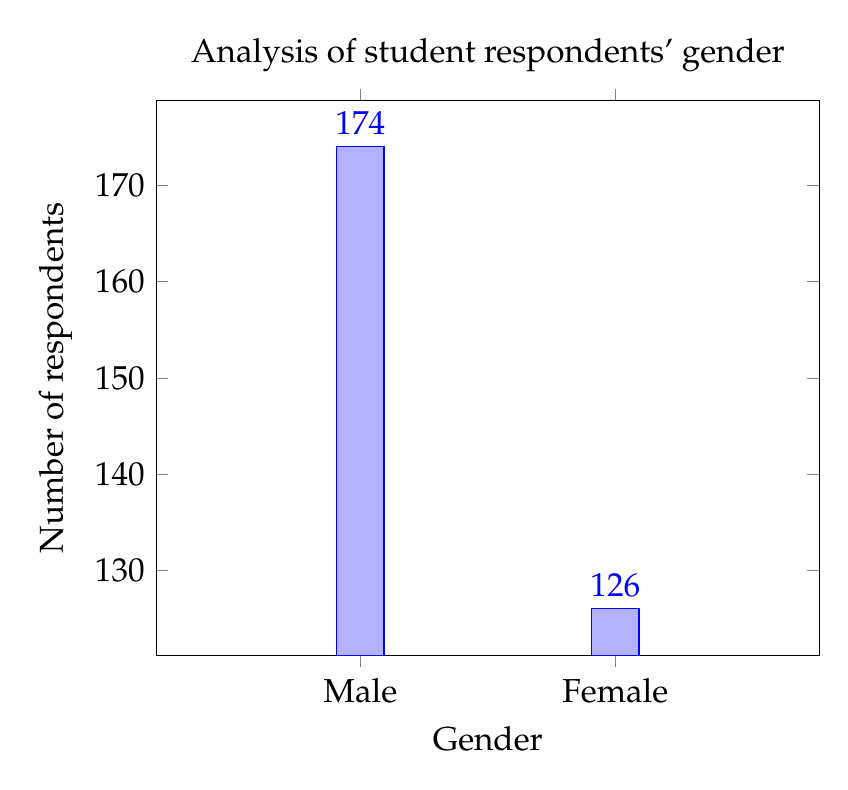
\begin{tikzpicture}
    \begin{axis}[
        title=Analysis of student respondents' gender,
        ybar,
        nodes near coords,
        bar width=0.6cm, 
        symbolic x coords={Male,Female},
        enlarge x limits=0.8,
        xtick=data,
        xlabel={Gender},
        ylabel={Number of respondents},
        xtick=data,  % add this option to remove extra tick labels
        legend style={
            at={(0.2)},
            anchor=south,
            column sep=1ex
        },
        width=10cm % set the width of the graph
    ]
    \addplot coordinates{(Male,174)(Female,126)};
   \end{axis}
   \end{tikzpicture}
\end{center}

\\
In the graph above, we observed that male students responded more than female students.


\noindent
\textbf{What college are you from?}
    \begin{center}
    
    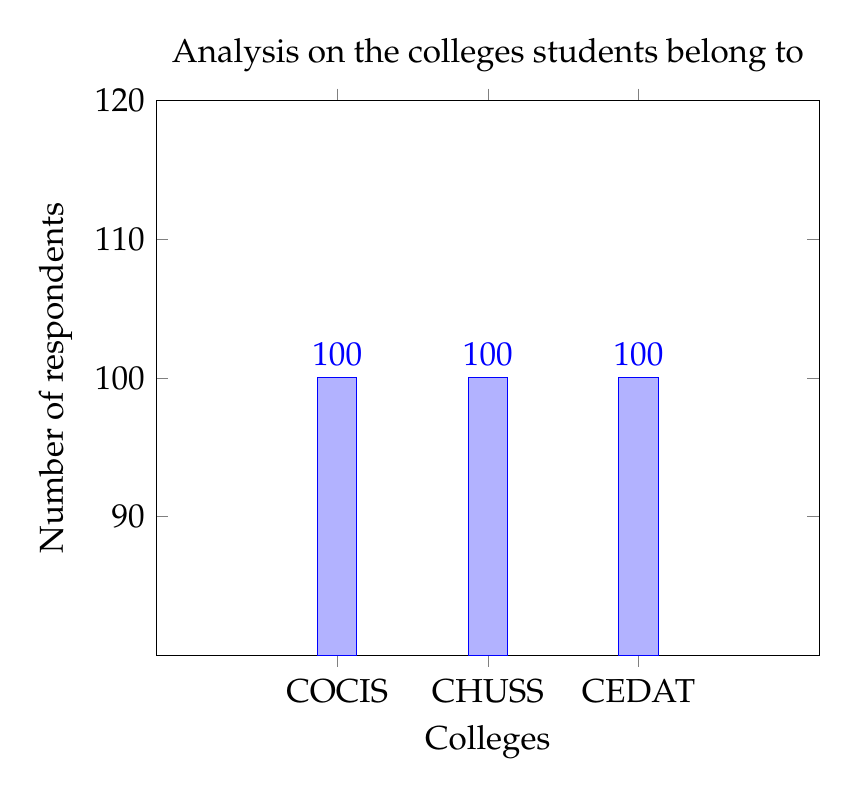
\begin{tikzpicture}
    \begin{axis}
[
title=Analysis on the colleges students belong to,
ybar,
nodes near coords, bar width=0.5cm, 
symbolic x coords={COCIS,CHUSS,CEDAT},
enlarge x limits=.6,
xlabel={Colleges},
ylabel={Number of respondents},
 xtick=data,  % add this option to remove extra tick labels
legend style={
at={(.2},
anchor=south,
column sep=1ex
},
width=10cm % set the width of the graph
]
\addplot coordinates{(COCIS,100)(CHUSS,100)(CEDAT,100)};
   \end{axis}
\end{tikzpicture}
\end{center}

In the graph above, we observe that we managed to get 100 responses from our target clusters.

\newpage
\subsubsection{Findings}

Our findings were categorized in form of questions answered by 300 respondents as follows.

\noindent
\textbf{Do you cook for yourself or buy ready-made food?}

\begin{figure}[h]
    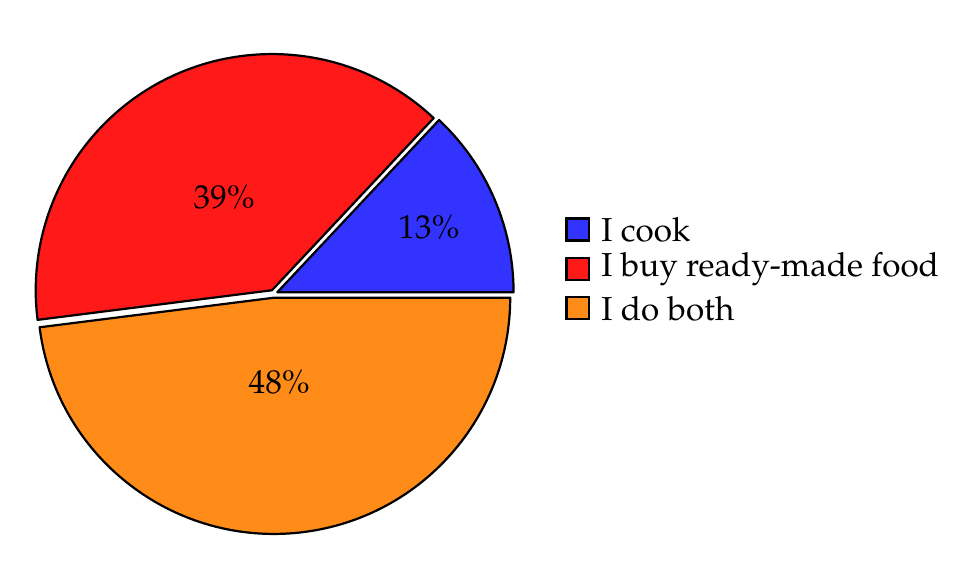
\begin{tikzpicture}
    \pie[
    color ={
    blue!80,
    red!90,
    orange!90},
    explode=0.05,
    text=legend
    ]
    {13/I cook,
    39/I buy ready-made food,
    48/I do both
   }
\end{tikzpicture}
\caption{Findings on the kind of food students take.}
\end{figure}

\noindent
\textbf{Do you have a consistent meal plan?}
    \begin{center}
    
    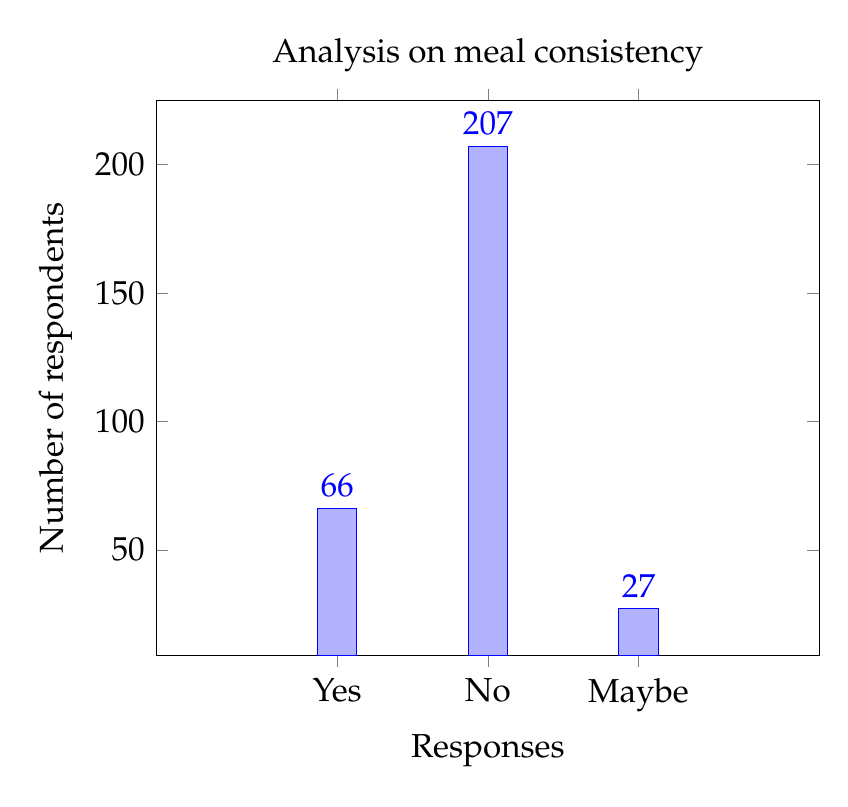
\begin{tikzpicture}
    \begin{axis}
[
title=Analysis on meal consistency,
ybar,
nodes near coords, bar width=0.5cm, 
symbolic x coords={Yes,No,Maybe},
enlarge x limits=.6,
xlabel={Responses},
ylabel={Number of respondents},
 xtick=data,  % add this option to remove extra tick labels
legend style={
at={(.2},
anchor=south,
column sep=1ex
},
width=10cm % set the width of the graph
]
\addplot coordinates{(Yes,66)(No,207)(Maybe,27)};
   \end{axis}
\end{tikzpicture}
\end{center}
\\
In graph above, we observed 207 students don't have consistent meal plans.


\noindent
\textbf{Do you a clear time frame for your meals?}
\begin{figure}[h]
    \centering
    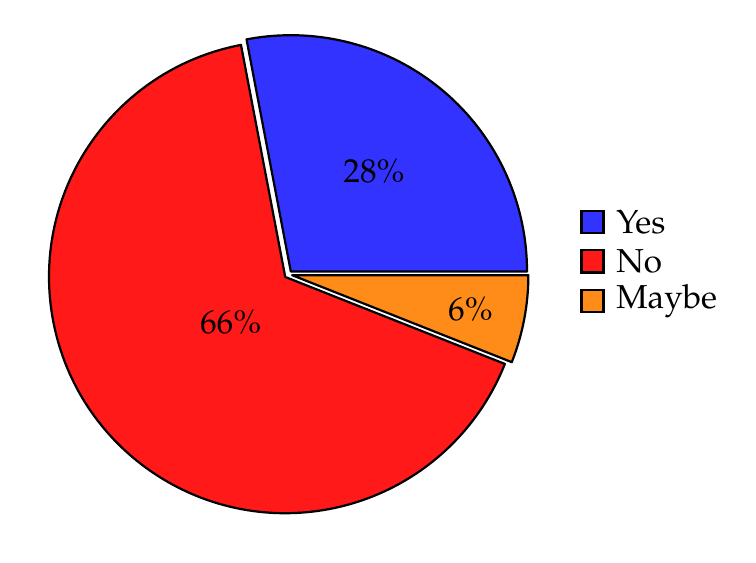
\begin{tikzpicture}
    \pie[
    color ={
    blue!80,
    red!90,
    orange!90},
    explode=0.05,
    text=legend
    ]
    {28/Yes,
    66/No,
    6/Maybe
   }
\end{tikzpicture}
\caption{Findings on the time frame of meals.}
\end{figure}
\\
In figure 2 above, we observed 66\% of the students don't have clear time frames for their meals.

\noindent
\textbf{How many meals do you have in a day?}
\begin{figure}[h]
    \centering
    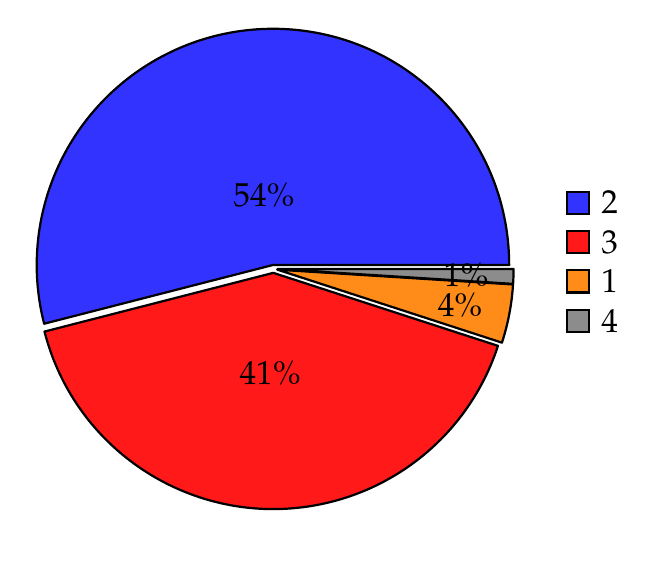
\begin{tikzpicture}
    \pie[
    color ={
    blue!80,
    red!90,
    orange!90,
    gray!90},
    explode=0.05,
    text=legend
    ]
    {54/2,
    41/3,
    4/1,
    1/4
   }
\end{tikzpicture}
\caption{Findings on the number of meals consumed in a day.}
\end{figure}
\\
In figure 3 above, we observed that over 54\% of the students have 2 meals a day.

\vspace{20pt}

\noindent
\textbf{Are these the same number of meals that you have been consuming since you joined the university?}
\begin{figure}[h]
    \centering
    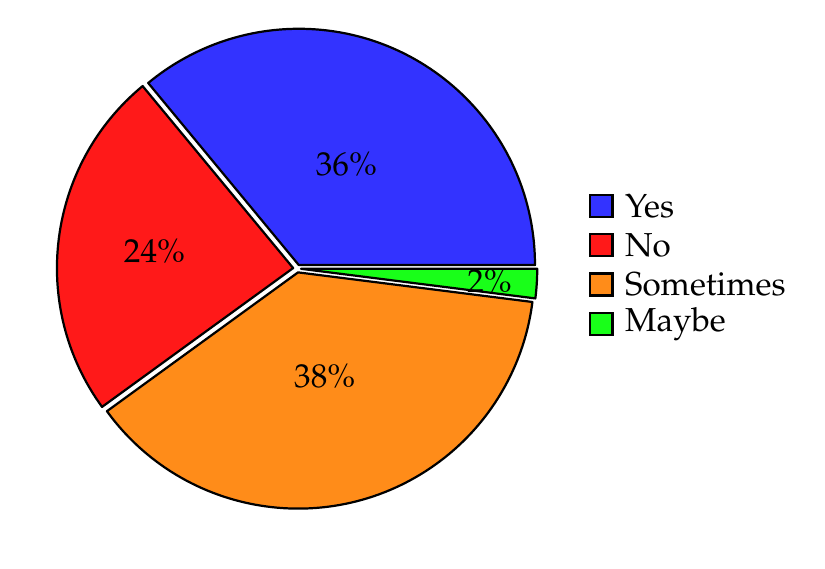
\begin{tikzpicture}
    \pie[
    color ={
    blue!80,
    red!90,
    orange!90,
    green!90},
    explode=0.05,
    text=legend
    ]
    {36/Yes,
    24/No,
    38/Sometimes,
    2/Maybe
   }
\end{tikzpicture}
\caption{Findings on the change in meals had since joining university.}
\end{figure}

In figure 4 above, we observed that 38\% of the students haven't had a big change in meals since joining university.

\vspace{30pt}

\noindent
Some of the reasons observed as to why students have had a change in the number of meals consumed since joining university are presented in the word cloud below.

\newpage
\begin{figure}[h]
  \centering
  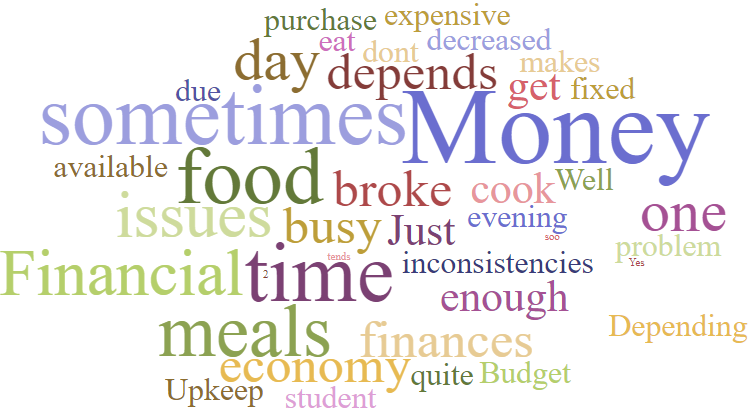
\includegraphics[width=360px]{images/wordcloud1.PNG}
  \caption{A word cloud showing the responses from students.}
\end{figure}

Using the word cloud above, we observed most students have had change in the number of meals mainly because of financial issues.

\noindent
\textbf{When did you join Makerere University?\\300 responses}
\begin{figure}[h]
    \centering
    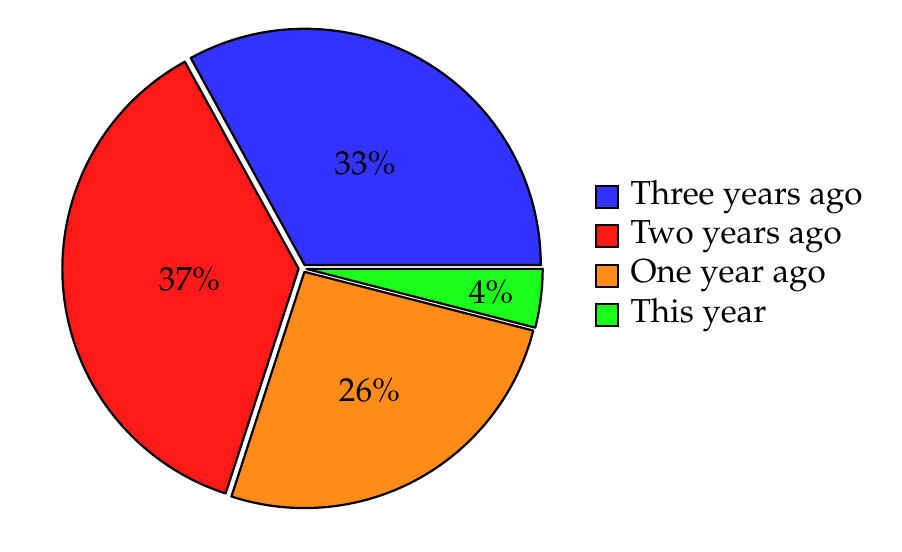
\begin{tikzpicture}
    \pie[
    color ={
    blue!80,
    red!90,
    orange!90,
    green! 90},
    explode=0.05,
    text=legend
    ]
    {33/Three years ago,
    37/Two years ago,
    26/One year ago,
    4/This year
   }
\end{tikzpicture}
\caption{Findings about when the students joined Makerere University.}
\end{figure}
\\
In figure 6 above, we observed that 37\% of the students joined Makerere University two years back.

\newpage
\noindent
\textbf{Qualitatively analyzed response from the Nutrionist.} 

\noindent The responses from the nutrionist from well-care clinic were qualitatively analyzed and these were the key points.

\noindent The nutrionist suggested that several factors that contribute to poor eating habits among university students include ignorance, economic standing, and lack of discipline. 

\vspace{10pt}

\noindent He also emphasized the importance of features that point towards mitigation, such as avoiding junk foods that directly invoke chronic illnesses and overly processed foods. Realistic options that promote sustainable work-life balance between healthy and junk foods were also suggested, with the inclusion  BMI readings and implementations that come along with the reading.

\vspace{10pt}

\noindent Regarding the target users of the proposed system, he recommended a focus on university students in the age bracket of 18-30, with a specific emphasis on males. When it comes to nutrients that make up a meal plan, he proposed including Vitamin B (fish, nuts), Magnesium (dark leaf vegetables), Vitamin K, Fibre, and Zinc (chia seeds). He stated proportions aren't necessary.

\vspace{10pt}

\noindent Regarding meal options, he advised not offering options with more than two starchy foods and adding in enough vegetables and fruits. He also suggested that a standard meal time of 8:00am-8:00pm and three meals in a day be implemented.

\vspace{10pt}

\noindent Overall, the nutrionist recommended making a flexible meal plan with short notes, many options, and graphics to cater for the needs of university students and promote healthy eating habits.

\vspace{40pt}

\noindent
\textbf{Qualitatively analyzed responses from Restuarant managers.}

\noindent
The responses from the two different restuarant managers were qualitatively analyzed and these were the key points noted.

\noindent
The Africa hall restaurant manager provided more detailed and diverse information, including insights on student preferences, cleanliness, ingredients, balanced diet, affordable prices, and favorite dishes. On the other hand, the COCIS restuarant manager 
 was more focused on customer complaints, limited space, and high prices of foodstuffs. Both respondents provided valuable perspectives on the restaurants and their operations, but the Africa hall retsuarant manager's response was more comprehensive.

\newpage
\section{System User Requirements}
The following are the users of the system:\\
\textbf{System Administrator.} System administrators have a higher understanding of how the system will work and have more privileges compared to other users of the system.\\
\textbf{Registered users.} These include Makerere University students.

\subsection{Functional and Non-functional Requirements}
\subsubsection{Functional Requirements.}
These requirements describe what the system should be based on the actor’s possible actions.\\
The functional requirements include;\\
\textbf{Registration Module.} The registration module allows all new users to register accounts.

\noindent
\textbf{Authentication Module.} The authentication module allows registered users to log in through their created accounts. 

\noindent
\textbf{Meal Planning Module.} The meal planner module creates and organizes meal schedules thereby allowing users to improve their diet by planning ahead for nutritious meals and tracking their calorie intake. From our findings, we observed that the majority of the respondents didn’t have a consistent meal plan. This justifies the need for implementing this feature in the system.

\noindent
\textbf{Timely Reminder Module.} The timely reminder module notifies the users when a particular meal is meant to be consumed according to the meal plan. Following our findings, the majority of the respondents lacked a clear time frame for ingesting particular meals.

\noindent
\textbf{Food suggestions Module.} The food suggestions module provides users with a variety of foods locally available to the populace. The findings indicated that most students cook food in addition to buying it in different circumstances. Implementing this module avails many options for the users to choose from.

\noindent
\textbf{Nutrition Analysis Module.} The nutrition analysis module analyzes food inputs and returns a response consisting of an array of different nutrients along with their food values.

\noindent
\textbf{BMI calculator Module.} The BMI calculator module informs the user of their height-to-weight ratio. Implementing this module helps users in the bid to track their calorie intake.

\subsubsection{Non-functional Requirements.}
These requirements specify the criteria that can be used to judge the operation of the system rather than specific behavior. They define system properties and the constraints of the system. The system must show software quality attributes such as accuracy, performance, cost security, and usability. The non-functional requirements include:

The system should be easy to maintain and adaptable to the users.

The system should provide forms of data capture during registration and login.

The system must provide login security at the application level.

The system should process user requests and return responses in time.

The system should be operational 24/7.

The system should be responsive i.e it should provide immediate feedback to users.

\subsection{System Requirements.}
\subsubsection{Software Requirements.}
Compatibility is a requirement to ensure that our system has the ability to run and perform required tasks properly. The table below points out the minimum requirements for the system.
\vspace{20pt}
\begin{table}[h]
    \centering
    \caption{Software requirements of the system.}
    
\begin{tabular}{|c|c|}
\hline
Software & Minimum System Requirements\\
 \hline  
 Browser & Google Chrome, Mozilla FireFox, Opera Mini, Edge\\
 \hline 
 Database & MySQL\\
 \hline 
 Operating System & All windows operating systems and\\ & some distros of Linux e.g Ubuntu\\
 \hline 
 Security  & System Authentication\\
 \hline
\end{tabular}

\label{tab: Software requirements of the system.}

\end{table}

\subsubsection{Hardware Requirements.}
The system required performing its specific tasks properly on hardware facilities. We carried research in different areas using different kinds of hardware facilities such as Laptops, smartphones and desktops to ascertain the right hardware for optimal system performance.

\vspace{10pt}
\begin{table}[h]
    \centering
    \caption{Hardware requirements of the system.}
    
    \begin{tabular}{|c|c|}
    \hline
    Hardware & Minimum System Requirements\\
     \hline  
     RAM & 2GB\\
     \hline 
     Disk Space & 10GB\\
     \hline
    \end{tabular}
    
    \label{tab: Software requirements of the system.}
\end{table}

%references
\newpage
\setlength\bibitemsep{3.0\itemsep}
\printbibliography


\newpage
\appendix
\renewcommand{\thesection}{} % Remove Numbering
\section{Appendix A: Students' Questionnaire.}

Here is the students questionnaire that was distributed among different colleges in Makerere University.

\vspace{30pt}
\begin{center}

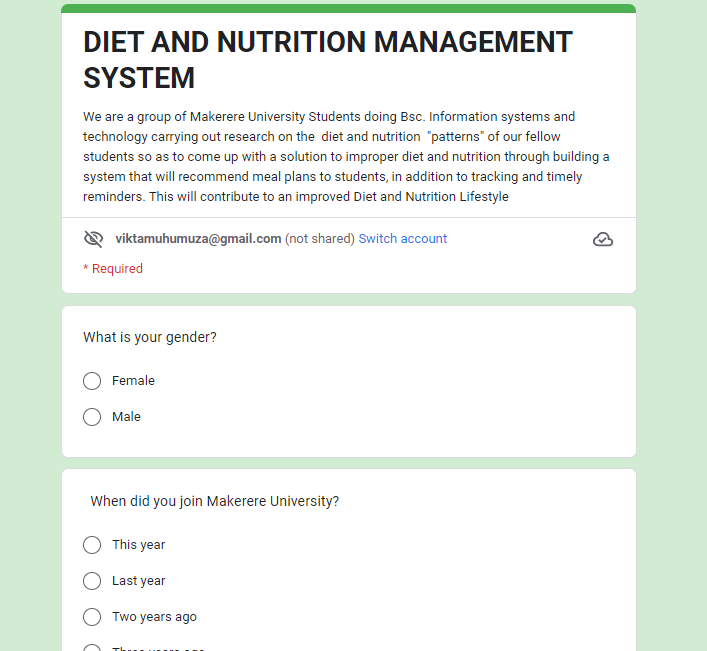
\includegraphics[width=280px]{images/questionnaire1.PNG}

 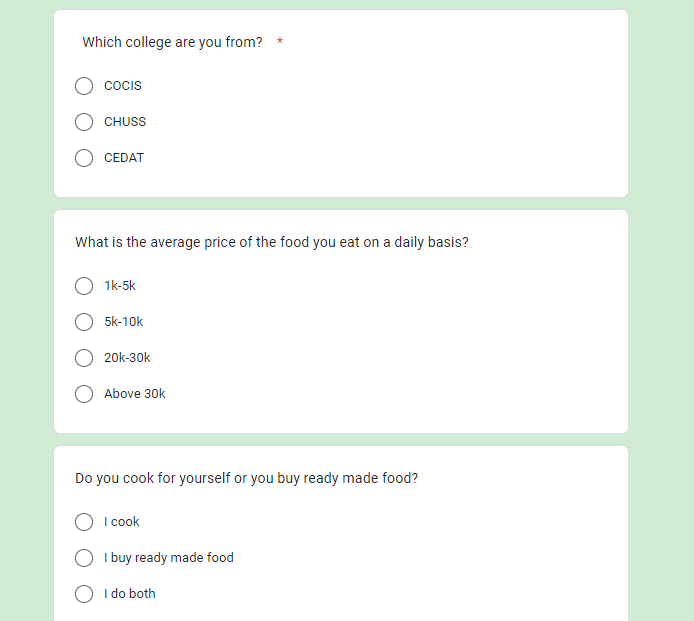
\includegraphics[width=280px]{images/questionnaire2.PNG}

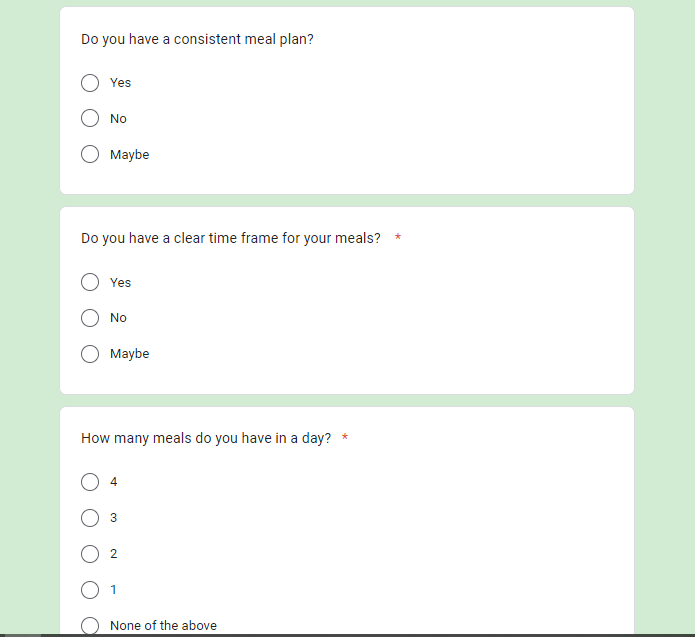
\includegraphics[width=280px]{images/questionnaire3.PNG} 

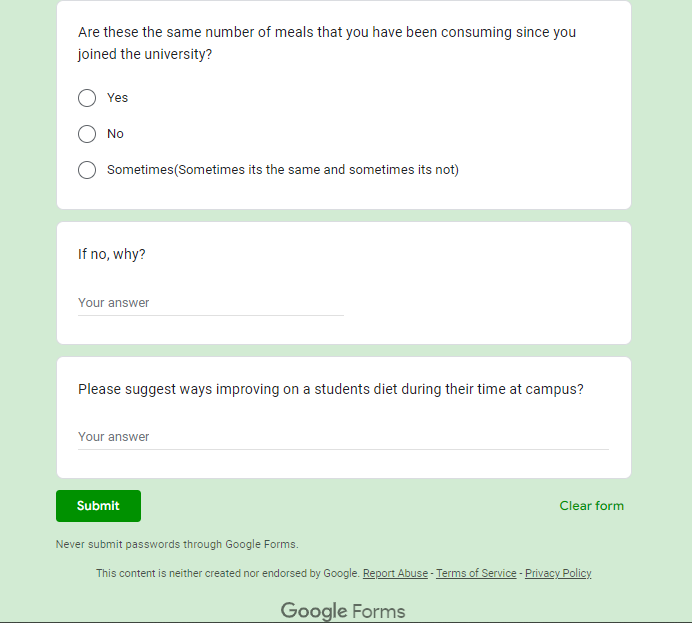
\includegraphics[width=280px]{images/questionnaire4.PNG} 
\end{center}

\newpage
\appendix
\renewcommand{\thesection}{} % Remove Numbering
\section{Appendix B: Doctor's Questionnaire.}

\vspace{30pt}
\begin{center}


\includegraphics[width=380px]{images/doctors1.PNG}

 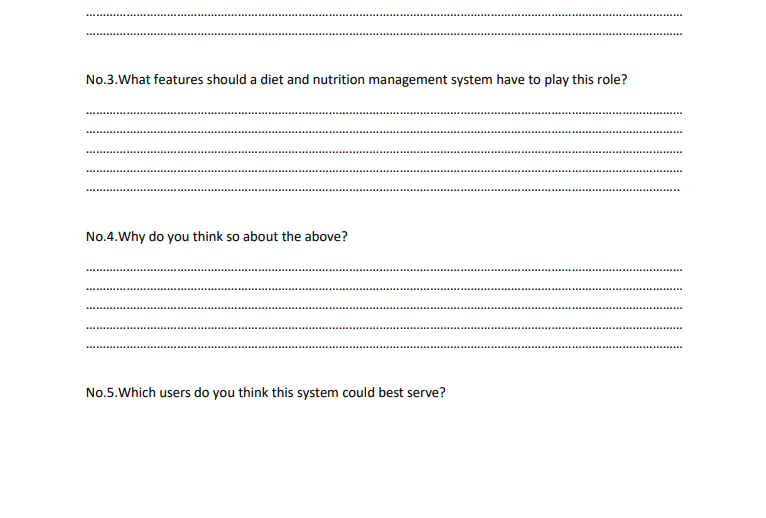
\includegraphics[width=380px]{images/doctors2.PNG}

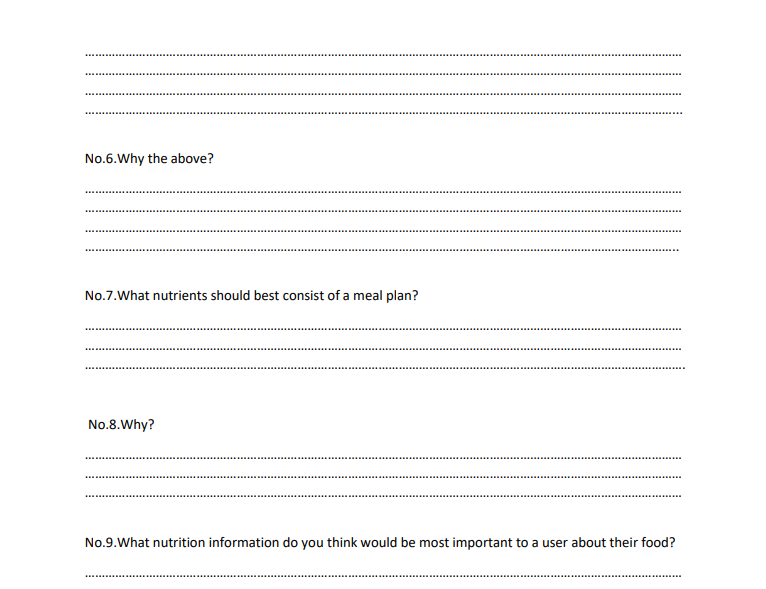
\includegraphics[width=380px]{images/doctors3.PNG} 

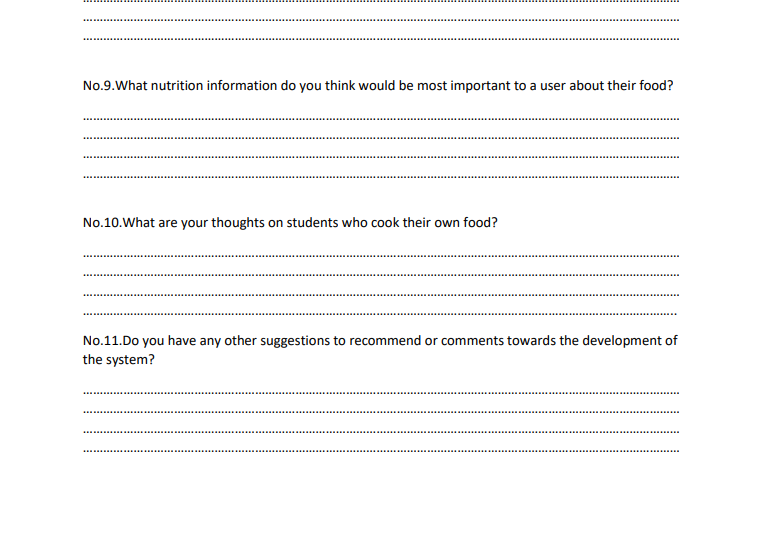
\includegraphics[width=380px]{images/doctors4.PNG} 
\end{center}

\newpage
\appendix
\renewcommand{\thesection}{} % Remove Numbering
\section{Appendix C: Restaurant managers' Questionnaire.}

\vspace{30pt}
\begin{center}


\includegraphics[width=380px]{images/restuarant1.PNG}

 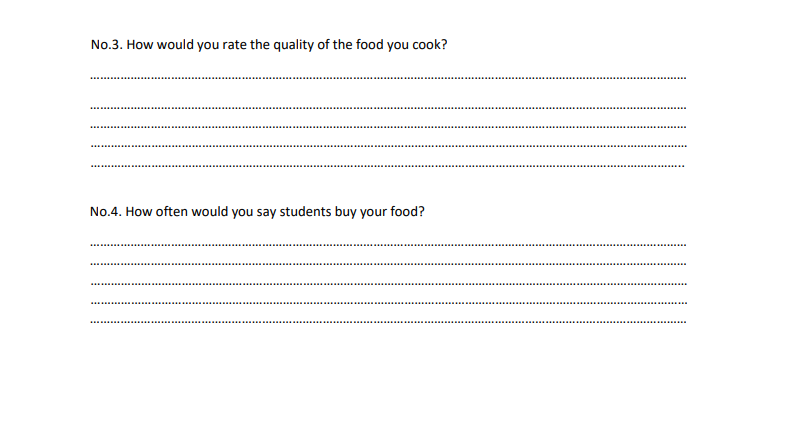
\includegraphics[width=380px]{images/restuarant2.PNG}

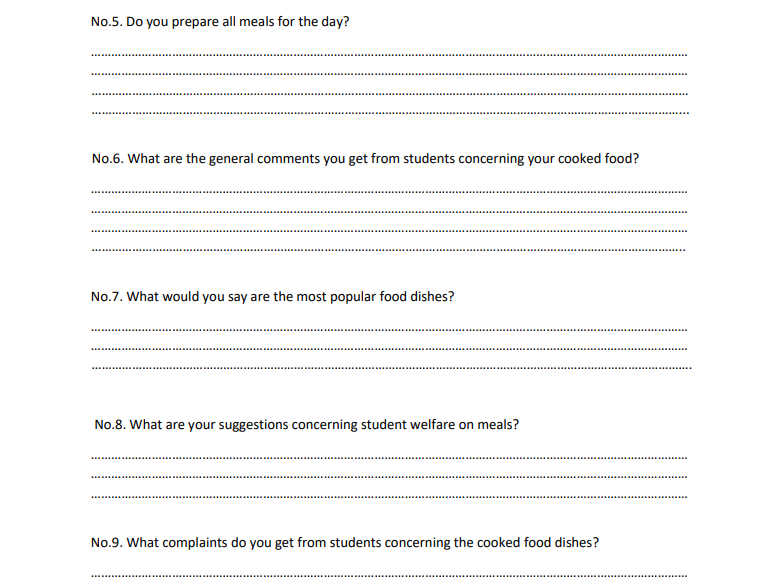
\includegraphics[width=380px]{images/restuarant3.PNG} 


\end{center}


\newpage
\appendix
\renewcommand{\thesection}{} % Remove Numbering
\section{Appendix D: Students' Responses. }

Some of the responses collected from students concerning the different questions asked in the questionnaire.

\vspace{30pt}
\begin{center}

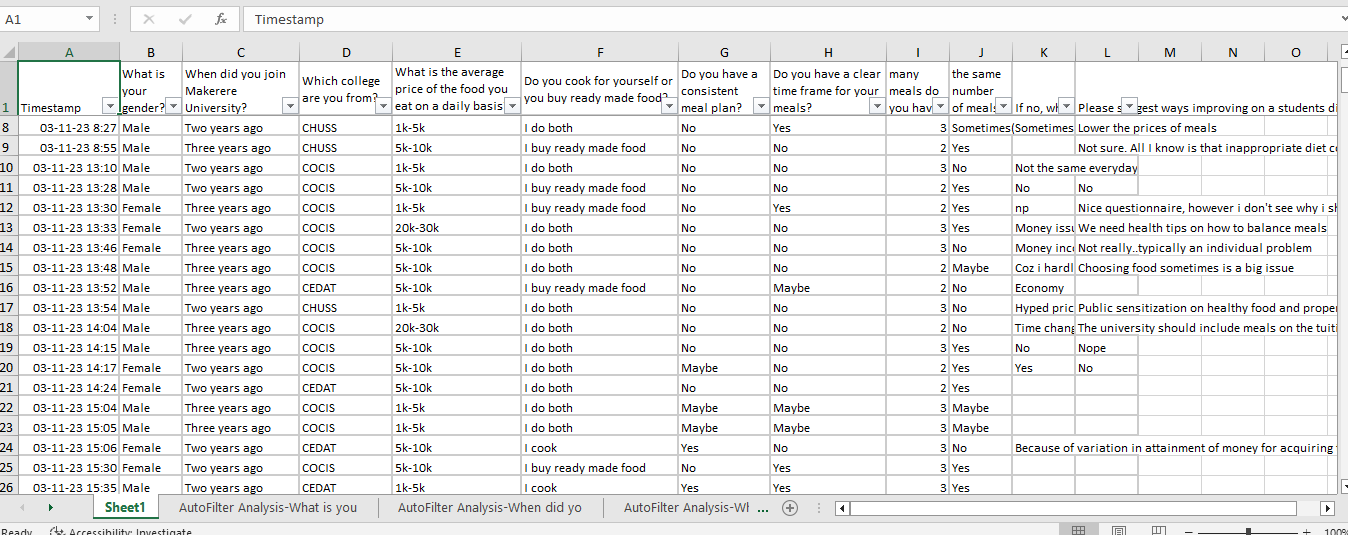
\includegraphics[width=460px]{images/data.PNG}\\
\vspace{30pt}
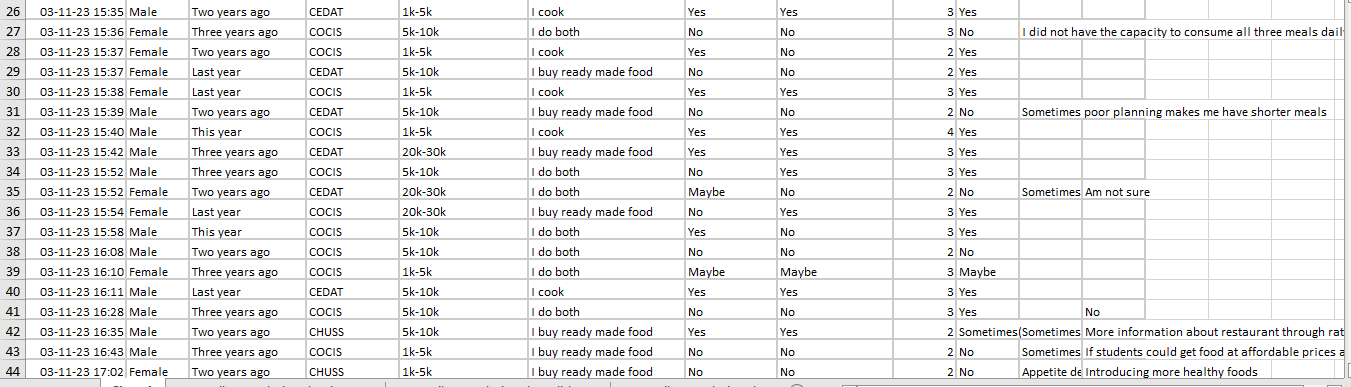
\includegraphics[width=460px]{images/data2.PNG}

\end{center}


\end{document}
